%%% Local Variables:
%%% mode: latex
%%% TeX-master: "../doc"
%%% coding: utf-8
%%% End:
% !TEX TS-program = pdflatexmk
% !TEX encoding = UTF-8 Unicode
% !TEX root = ../doc.tex

This sections explains the fundamental technologies and achievements from previous projects which have been applied in the project.

\section{Technological prototype}
As mentioned in chapter \ref{Initial position}, a technological prototype for the ATP has already been developed in a bachelor thesis during the previous semester.
The prototype has been realised as a locally running application using the ASP.NET Core Blazor framework \cite{bachelorarbeit_Egger_Verstappen_page4}. The application
fetches time data from Toggl Track via the Toggl Track API and relies on Local Storage for storing the application state. The graphical user interface has been designed
with elements from the Bootstrap toolkit. Charts.js is used to display graphs and charts. The application is made available as a Docker image which can be downloaded
from the GitHub Container Registry. As to software testing, unit tests for the part managing the communication between the application and Toggl have been implemented and
can be run automatically via GitHub Actions. \cite{bachelorarbeit_Egger_Verstappen_page23-25}.

The different features, however, have not been fully implemented yet. The charts display dummy data instead of real time data, as shown in figure \ref{figure1}. The tracked time data can be retrieved
from Toggl, but no further action is applied to it. Local Storage is not considered to be suitable for application data storage on the long term. Further possible
enhancements include localisation, accessing other APIs and not just Toggl, different installation and update strategies as well as additional automated tests like UI
tests and integration tests \cite{bachelorarbeit_Egger_Verstappen_page26-27}.

\begin{figure}[H]
\centering
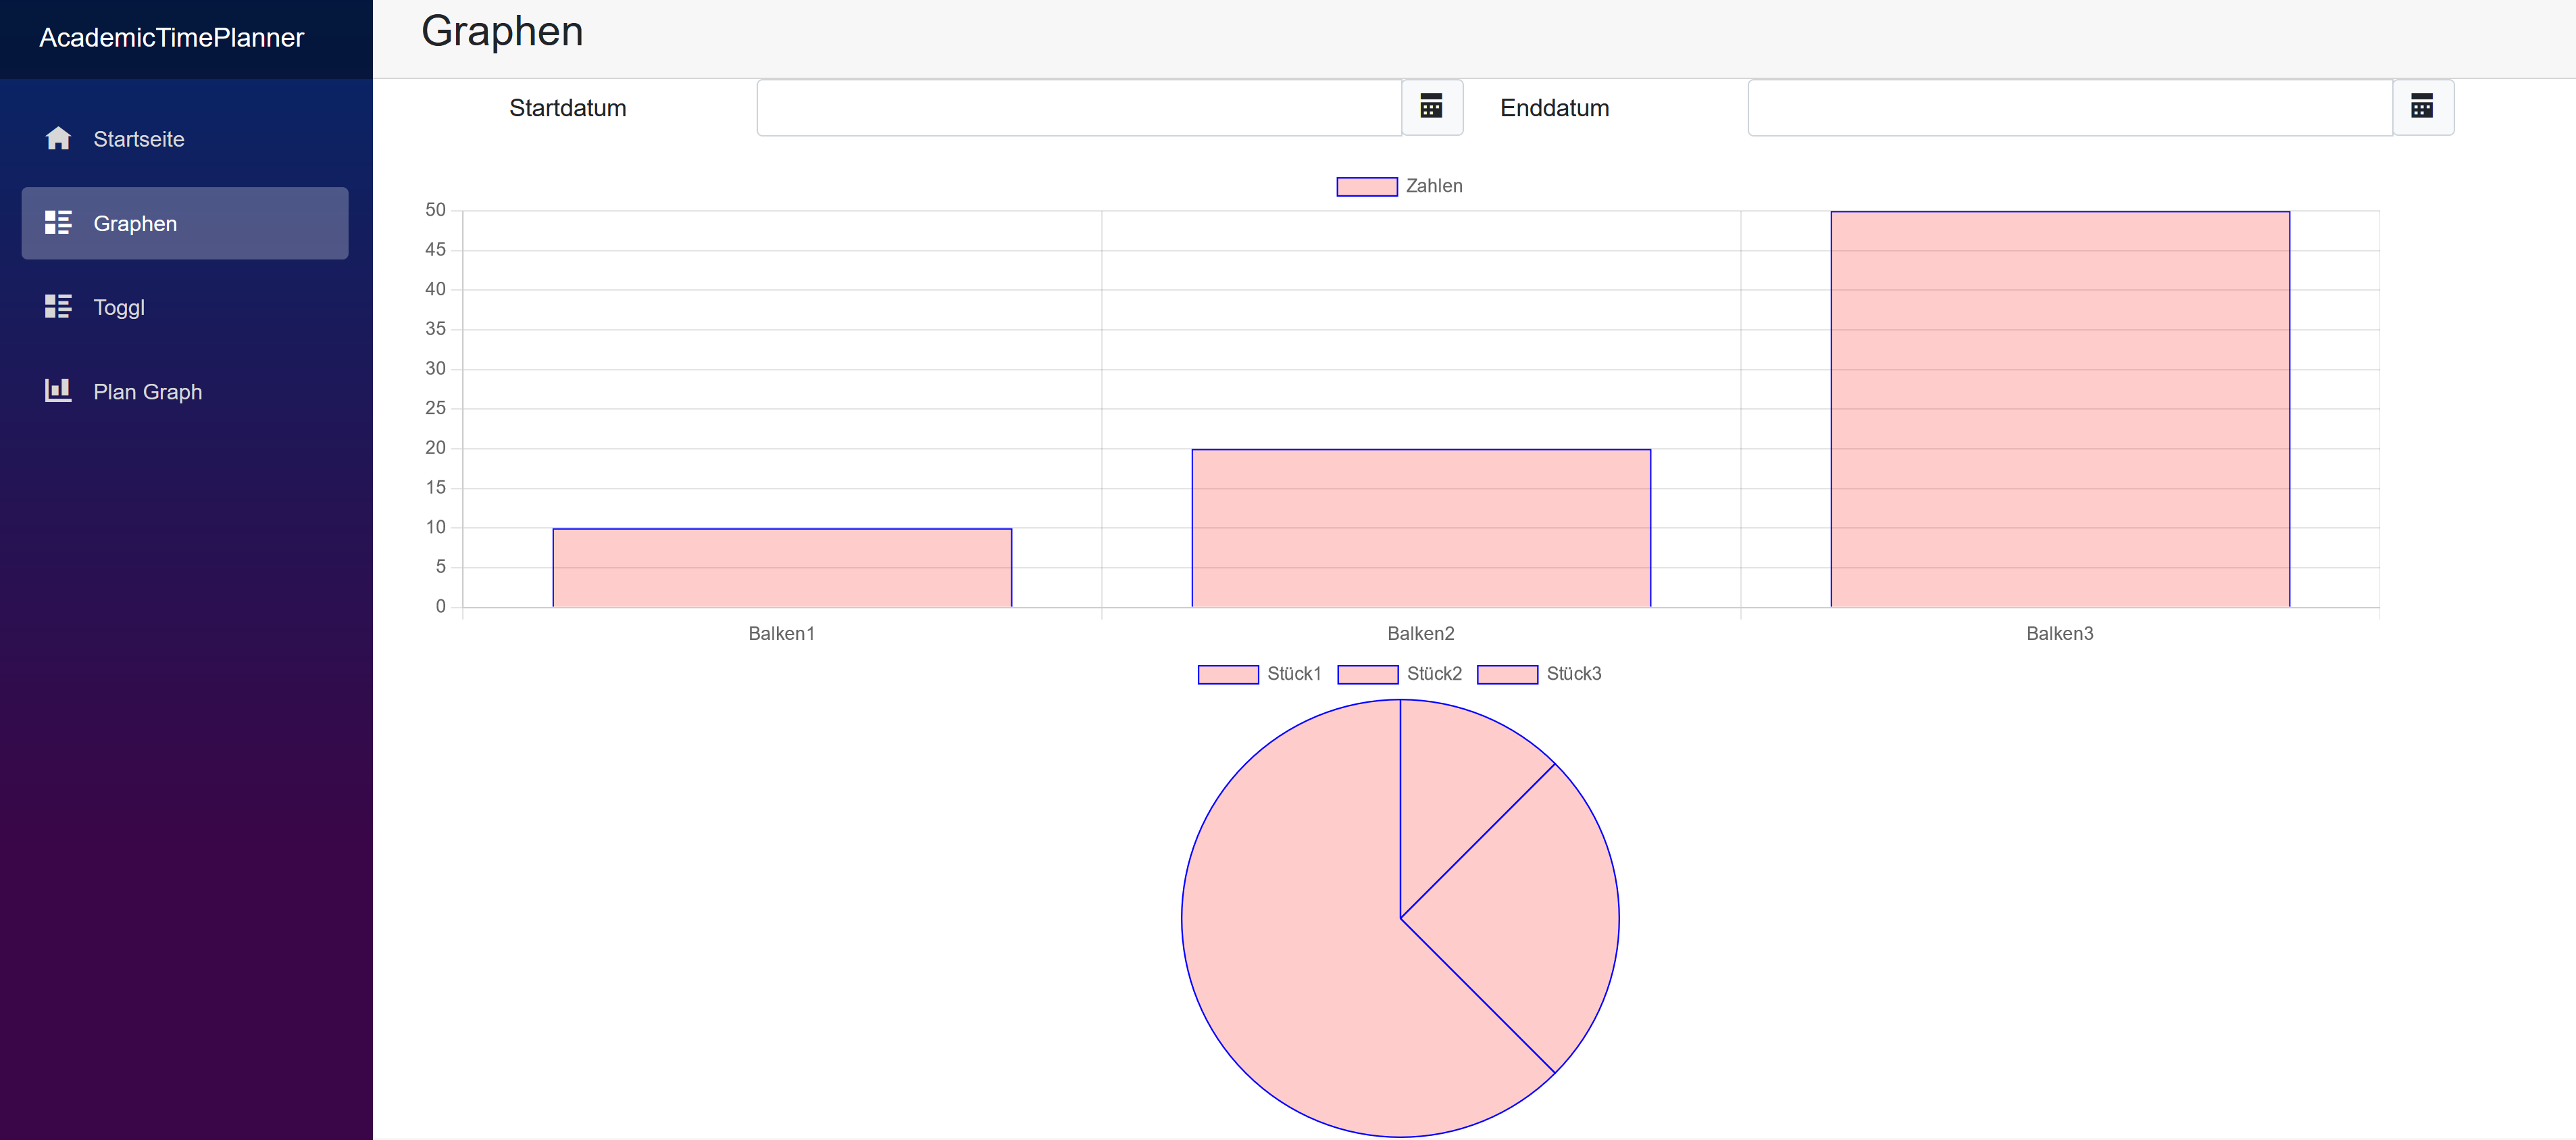
\includegraphics[width=1.0\columnwidth]{figure1_prototype_charts}
\caption{ATP prototype displaying dummy charts}
\label{figure1}
\end{figure}